% !TeX spellcheck = de_CH
% !TeX encoding = UTF-8
% !TeX root = ../presentation.tex

\section{Einführung}

\begin{frame}{Um was geht es?}
\begin{itemize}
\item<1-> Verhalten von Mischungen zweier Materialien (Phasen) über die Zeit
\item<2-> Ursprüngliche Anwendung war ein theoretisches Modell für die Entmischung von binären Legierungen
\end{itemize}
\uncover<3->{
\begin{figure}
\centering
\begin{subfigure}{0.18\textwidth}
\centering

\includegraphics[width=\textwidth]{images/ch_sim/0.pdf}
\caption{$t = 0\,\tau$}
\end{subfigure}
\qquad
\begin{subfigure}{0.18\textwidth}
\centering
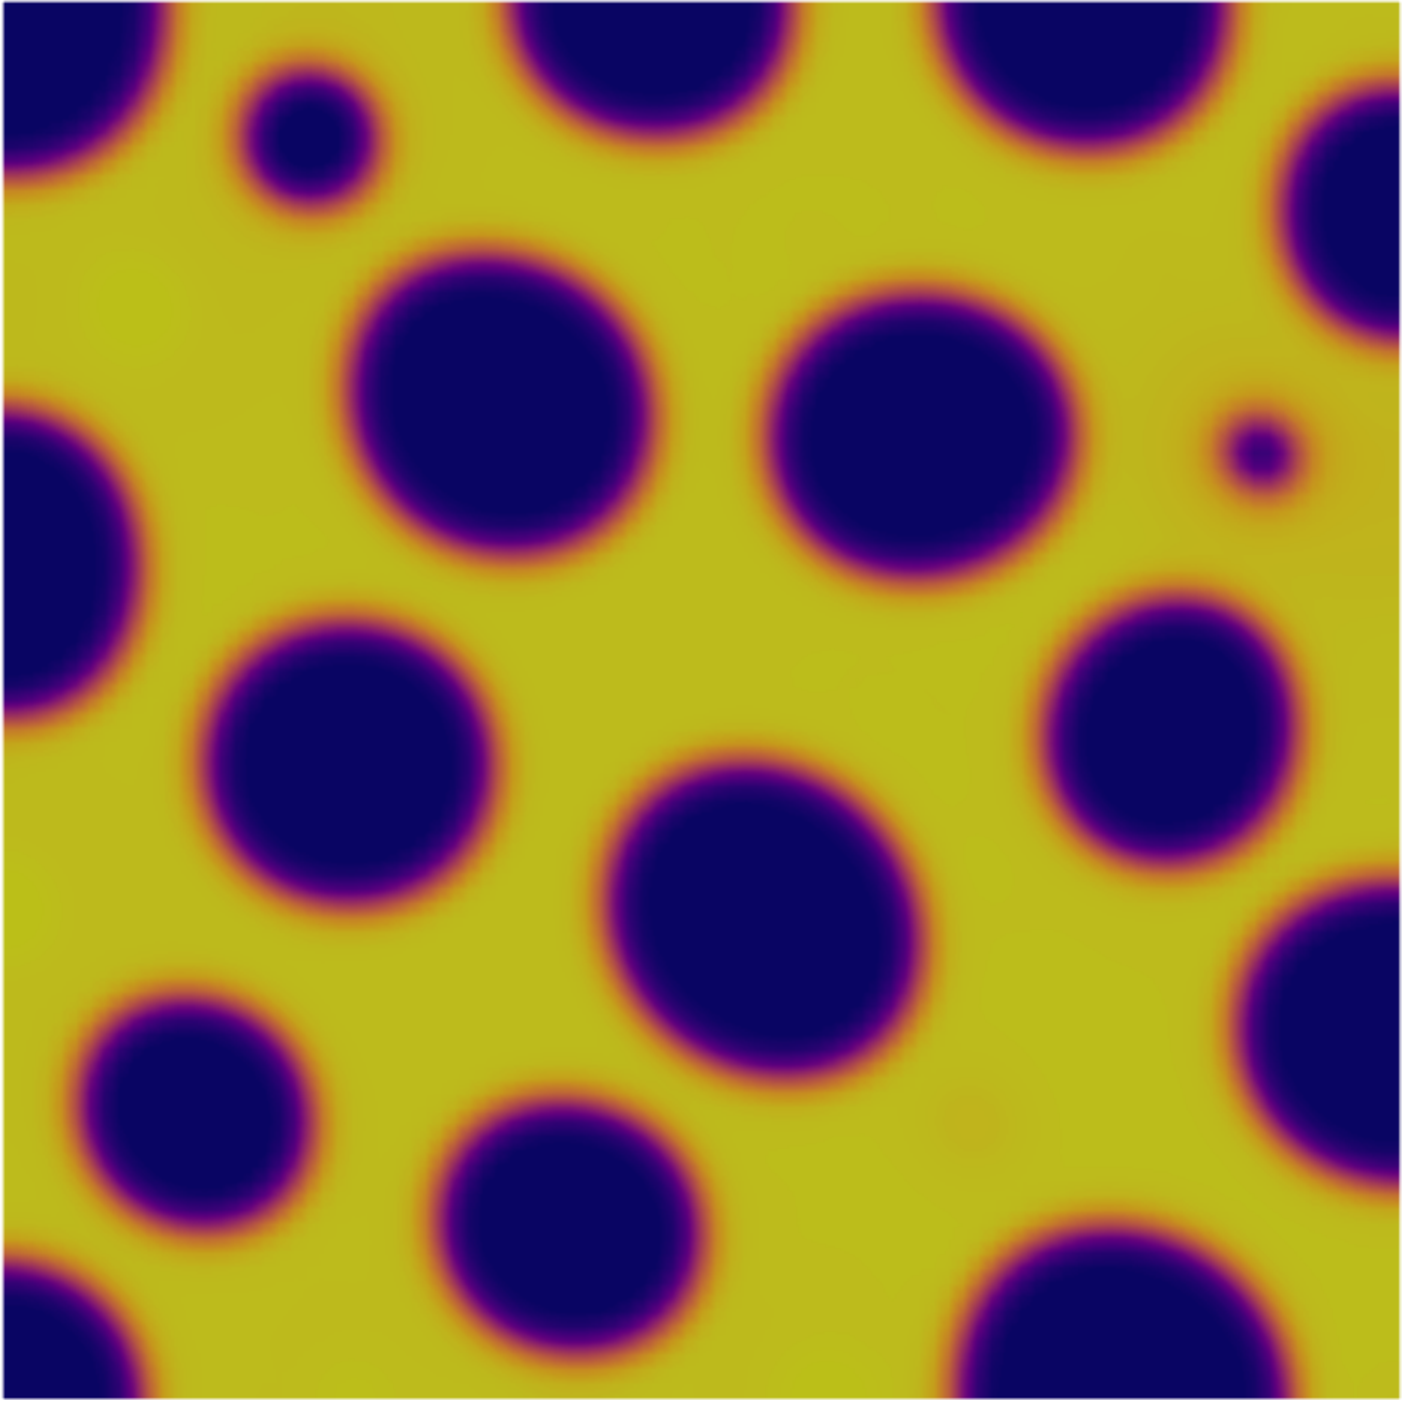
\includegraphics[width=\textwidth]{images/ch_sim/300.pdf}
\caption{$t = 300\,\tau$}
\end{subfigure}
\caption{Beispiel spinodaler Entmischung}
\end{figure}
}
\end{frame}

\begin{frame}{Definitionen}
\begin{itemize}
\item<+-> $N_A$ lokale Stoffmenge von Stoff A, $N_A > 0$
\item<+-> $N_B$ lokale Stoffmenge von Stoff B, $N_B > 0$
\item<+-> $c$ lokale Konzentration von Stoff B
\begin{align*}
c
=
\frac{N_B}{N_A + N_B}
\quad \Rightarrow \quad c \in [0, 1]
\end{align*}
\item<+-> $F(c)$ freie Energie pro Molekül eines homogenen Gemisches
(wir betrachten diese Funktion als gegeben)
\end{itemize}
\end{frame}

% \begin{frame}{Was}
%   frame
% \end{frame}
